% ----------------------------------------
% Proof of concept
% ----------------------------------------

\chapter{Proof of concept}
\label{ch:proof-of-concept}

In this chapter, a proof-of-concept solution around a specific business case is
created to demonstrate the practical use of the \gls{mfa} pattern.

As was made apparent in section \fullref{ssec:mf-implementation-patterns}, there
are several different ways of conceptualizing and creating \gls{microfrontend}
solutions. This \gls{poc} will focus on \textbf{universal composition}, to be
able to enable \textbf{\gls{pe}} of the resulting web application. The desired
solution ideally uses an exclusive \textbf{.NET approach} (i.e. using
exclusively technologies within the .NET ecosystem), and has \textbf{run-time
integration} with dynamic (lazy) loading capabilities.


\section{Domain}
\subsection{Description}

This \gls{poc} is centered around an e-commerce domain. To make the
business case more specific and tangible, the case was formulated as
follows:

\begin{quote}
  The creation of a web application for an online store dedicated to selling
  tabletop games (board games, card games, ...).
\end{quote}

This encompasses the following functionalities:
\begin{itemize}
  \item Browse games
  \item View game details
  \item Order games
\end{itemize}

This domain was chosen because the technical needs of e-commerce solutions tend
to overlap with the set-out desired characteristics of the proof-of-concept
application. In a real world scenario, obviously the reverse process would be
necessary, and one would have to  pick the best suiting implementation pattern
for the case at hand. 

The universal rendering will make sure the application has a faster initial load
and better \gls{seo} than a purely client-side rendered application, while
maintaining a highly dynamic nature.

\subsection{Decomposition into microfrontends}

According to \textcite{Rappl_2021}, the domain decomposition strategy is a
crucial foundation for determining the architecture of the \gls{microfrontend}
solution. In a real company context, both technical and organizational factors
need to be considered to be able to split up the domain. For this \gls{poc}, the
following modules were chosen:

\begin{itemize}
  \item The \textit{Discover} \gls{microfrontend}, containing the product
  overviews and product details.
  \item The \textit{Order} \gls{microfrontend}, containing everything necessary
  for ordering products.
\end{itemize}

\section{Architecture}

Using the domain decomposition results, the overall architecture of the solution
can be determined. An overview is given in Figure~\ref{fig:poc-architecture}. It
mainly consists of 3 parts:
\begin{itemize}
  \item The \textit{Discover} \gls{microfrontend}
  \item The \textit{Order} \gls{microfrontend}
  \item The \gls{appshell} where these \glsplural{microfrontend} will
  get integrated into.
\end{itemize}
 

\begin{figure}
  \centering
  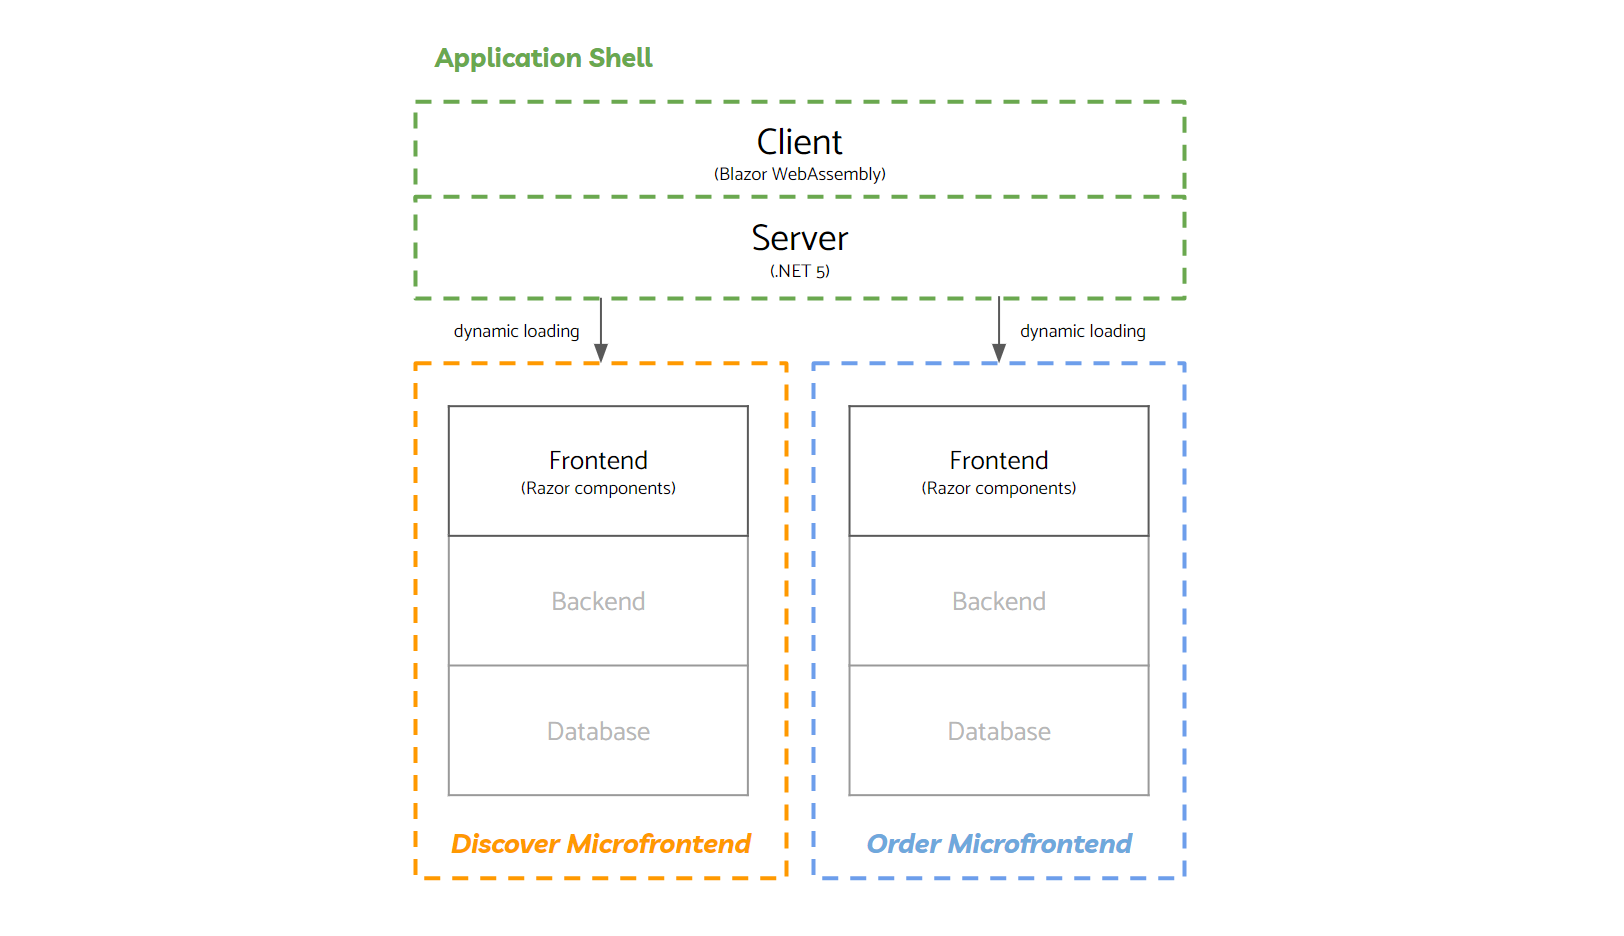
\includegraphics[width=0.8\textwidth]{poc-architecture}
  \caption[Architecture overview for proof-of-concept solution]{The architecture
  overview for the proof-of-concept solution. In the \glsplural{microfrontend},
  only the \gls{frontend} has been implemented in the \gls{poc}, while the other
  elements were mocked using in-memory solutions for demonstration purposes.  
  }
  \label{fig:poc-architecture}
\end{figure}

\subsection{Composition structure}
\label{ssec:poc-composition}

A visual overview for the component and page composition for the \gls{poc}
application is shown in Figure~\ref{fig:poc-components}. Pages are registered on
a certain route and fragments are registed into a slot (with a unique name) in
another \gls{microfrontend} or the \gls{appshell}.

\begin{sidewaysfigure}
  \centering
  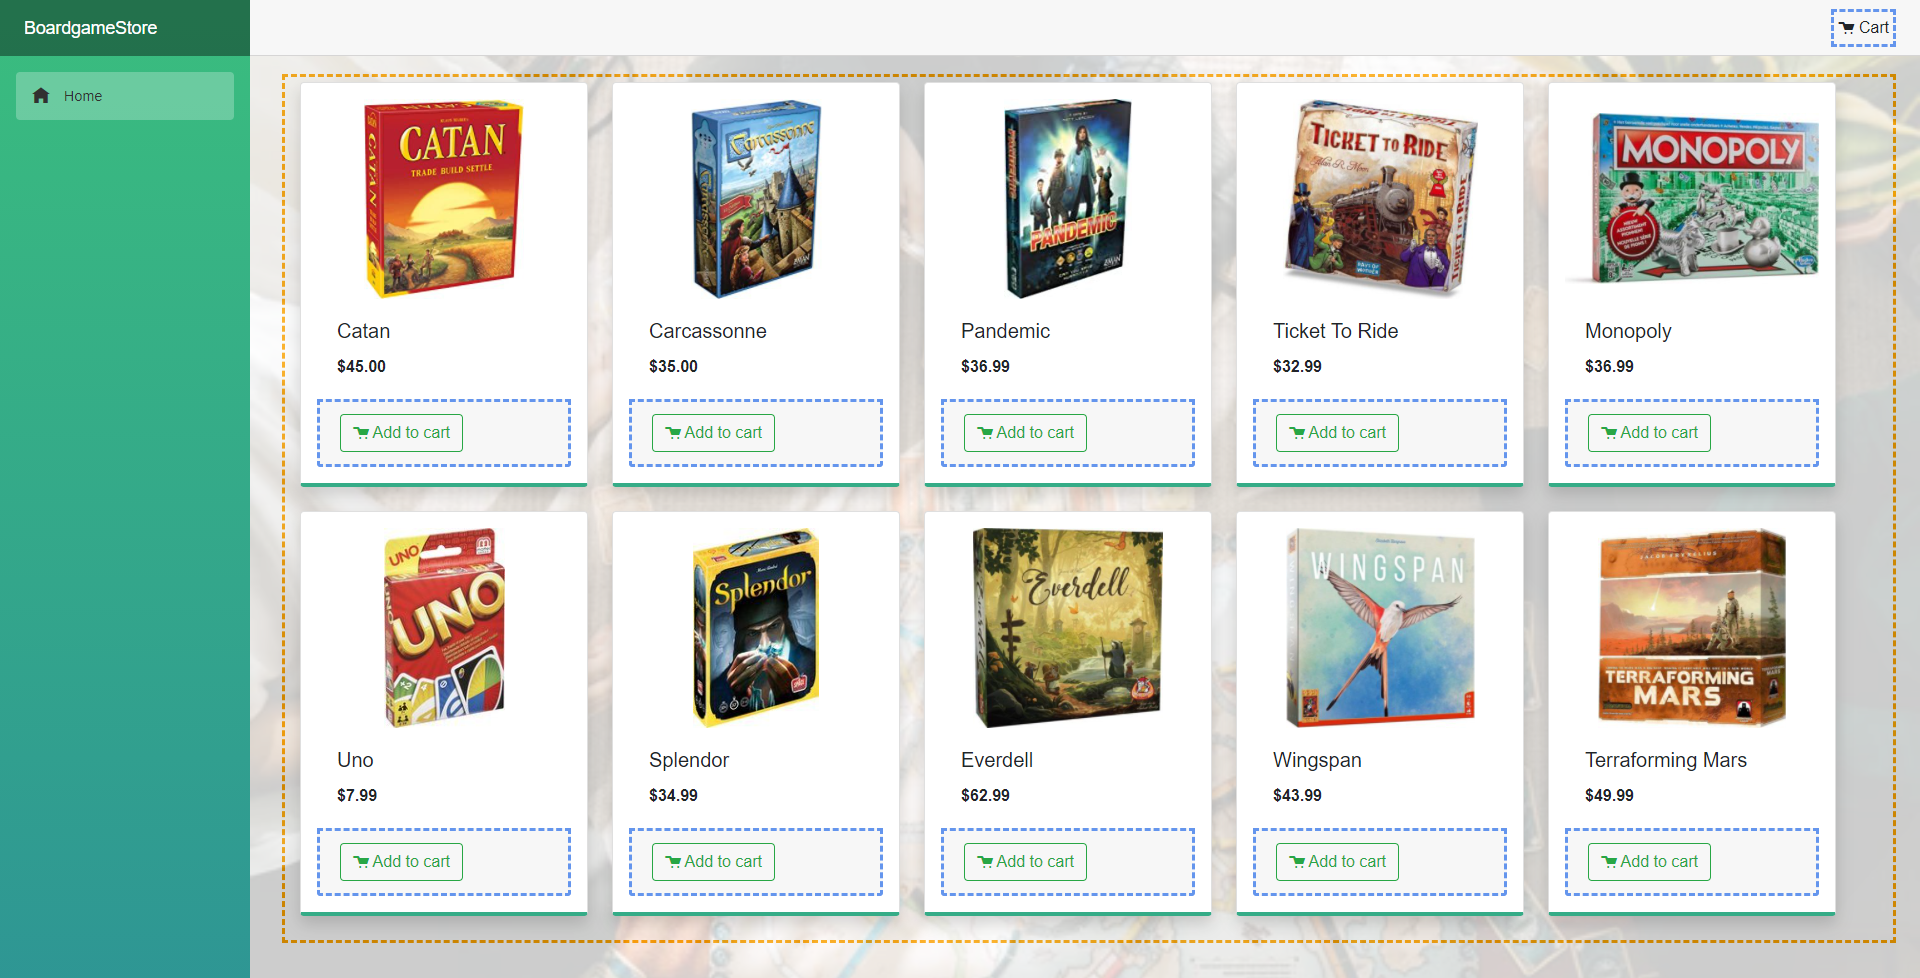
\includegraphics[width=\textwidth]{poc-components}
  \caption[Visual overview for proof-of-concept solution]{A visual overview for
  the component and page composition for the \gls{poc} application. The colored
  dashed lines indicate the sources of the components (blue for
  \textit{``Order''} \gls{microfrontend}, orange for \textit{``Discover''}).}
  \label{fig:poc-components}
\end{sidewaysfigure}

\begin{keeptogether}
  A summary of the components each \gls{microfrontend} exposes is shown below:
  \begin{framed}
    \textit{Discover}  \gls{microfrontend}:
      \begin{itemize}
        \item[] Pages
        \begin{itemize}
          \item \texttt{GameDetails} with route \texttt{/game?id=\{id\}}
        \end{itemize}
        \item[] Fragments
        \begin{itemize}
          \item \texttt{GameOverview} for slot \texttt{homepage}
        \end{itemize}
      \end{itemize}
    \textit{Order} \gls{microfrontend}:
      \begin{itemize}
        \item[] Pages
        \begin{itemize}
          \item \texttt{CartOverview} with route \texttt{/cart}
          \item \texttt{OrderConfirmation} with route \texttt{/orderconfirmation}
        \end{itemize}
        \item[] Fragments
        \begin{itemize}
          \item \texttt{AddToCartButton} for slot \texttt{game-actions}
          \item \texttt{CartLink} for slot \texttt{top-row-items}
        \end{itemize}
      \end{itemize}
  \end{framed} 
\end{keeptogether}


\section{Development}
\label{sec:poc-development}

In what follows, more information about the development of the \gls{poc}
solution will be given. This explanation is accompanied by code that can be
found at
\begin{quote}
   \url{https://github.com/DanteDeRuwe/bachelor-thesis-code}.
\end{quote}

\subsection{Preparation}

An ASP.NET hosted Blazor \gls{wasm} project was created. This can be done via
the .NET \gls{cli}:

\begin{minted}{console}
  $ dotnet new blazorwasm --hosted
\end{minted}

This solution will serve as the \gls{appshell} of the \gls{microfrontend}
application. It consists of a client and a server part.

Next, pre-rendering was enabled in the \gls{appshell}, using a strategy outlined
in a blogpost by Jon Hilton
\footnote{\url{https://jonhilton.net/blazor-wasm-prerendering/}}.

\subsection{Process and results}

\subsubsection{The framework library}

To be able to dynamically integrate the \glsplural{microfrontend} into the
\gls{appshell} at runtime, it is useful to create a baseline framework with
various utilities and reusable components.

This is the goal of the
\texttt{MicrofrontendFramework.Blazor}\hreffootnote{https://github.com/DanteDeRuwe/bachelor-thesis-code/tree/main/src/framework/MicrofrontendFramework.Blazor}
project. It has the following functionalities:

\begin{itemize}
  \item Fragment rendering: the framework exposes a
  \mintinline{csharp}|[Fragment]| attribute to register a component as a
  fragment with a custom name. It then also exposes a
  \mintinline{html}|<Fragment/>| component that is used from the \gls{appshell}
  or other \glsplural{microfrontend} to render a fragment by name.
  \item Routing: the framework exposes a \mintinline{html}|<DynamicRouter/>|
  component that can be used in stead of the default Blazor router to render the
  corresponding component dynamically
  \item Component registration and \gls{di}: This functionality is exposed as
  via an extension method called \mintinline{csharp}|AddMicroFrontends| that,
  given a collection of loaded assemblies, can extract a collection of all
  components, and register this collection onto the \gls{di} container. It also
  will register the services that these \glsplural{microfrontend} need onto the
  provided service collection.\footnote{It does this by looking up a
  \texttt{Microfrontend} class in the \gls{microfrontend} and reflectively
  calling its \texttt{Configure} method. See
  \href{https://github.com/DanteDeRuwe/bachelor-thesis-code/blob/main/src/framework/MicrofrontendFramework.Blazor/Extensions.cs\#L30-L39}{MicrofrontendFramework.Blazor/Extensions.cs:30-39}}
\end{itemize}

\subsubsection[The application shell]{The \gls{appshell}}

The main responsibility of the \gls{appshell} is to compose the
\gls{microfrontend} components and integrate the \glsplural{microfrontend} into
itself. This includes executing the functionalities present in the framework
library such as \textbf{routing} and \textbf{fragment rendering}. Before it can
make use of the \mintinline{csharp}|AddMicroFrontends| extension method, it
should dynamically load the \gls{microfrontend} assemblies to be able to pass these as
an argument.

On the server side, as by way of proof of concept, the \gls{appshell} fetches
the \gls{microfrontend} assemblies from disk, acting as an ad hoc \gls{cdn}. The
server then also exposes the file paths via a \gls{restful}
\gls{api}.\footnote{In a real-world scenario, these responsibilities would
probably be assigned to a dedicated service.} From the client side, the file
paths are fetched via an \gls{http} call to the server \gls{api}, and the files
themselves are then fetched via their paths.

The assemblies are stored in \gls{dll} files. To also enable the debugging of
the \glsplural{microfrontend}, another type of file is also needed: the
\gls{pdb} files. As mentioned before, these are also called \textit{symbol}
files, and they are the link between the debugger and the source code
\autocite{Microsoft_2021}.

On both the server and the client side, each assembly and symbol definition can
be loaded in memory using the default \mintinline{csharp}|AssemblyLoadContext|:

\begin{minted}{csharp}
AssemblyLoadContext.Default.LoadFromStream(dllStream, pdbStream);
\end{minted}

Once these are loaded, they can be passed on to the aforementioned
\mintinline{csharp}|AddMicroFrontends| extension method originating from the
framework project.

Next to fragment rendering, dynamic loading and routing, the \gls{appshell} also
has responsibility over some {\textbf{shared capabilities} such as navigation,
and basic \textbf{layout}.
 
\subsubsection{The microfrontends}

In this \gls{poc} solution, every \gls{microfrontend} is just a Razor class
library exposing a certain set of pages and fragments. An overview of these
exposed elements was shown in \fullref{ssec:poc-composition}. These exposed
components are then picked up by the \gls{appshell} (using the framework
library) for integration.

Each \gls{microfrontend} is also an independent owner of its own data. They are
not strongly coupled to the \gls{appshell} in any way, and only use the
framework library to be able to expose fragments and use placeholder slots for
for the \gls{appshell} to integrate other fragments into.